\chapter{Knowledge Distillation}
\label{part_2}
\acrfull{kd} is a frugal AI technique known to provide great results. Using the results of a large model at training time, a smaller model can achieve performances which tends towards that of the large model. This chapter focuses on applying \acrshort{kd} to \acrshort{lic}. In order to do that, we first experiment with \acrshort{kd} on auto-encoders for image reconstruction. After achieving satisfactory results, we proceed in implementing \acrshort{kd} for \acrshort{lic}.

\section{Knowledge Distillation for Image Reconstrution}
As explained by Ballé et al. in \cite{ballé2018variationalimagecompressionscale}, \acrshort{vae}s are very similar to \acrshort{lic} architectures in the sense that they both have some sort of analysis transformation to transfer the input signal to a low dimensional latent space and an approximate of this analysis transform (the synthesis transform) to transfer the latent representation back to the signal space. However, in \cite{minnen2018jointautoregressivehierarchicalpriors}, the authors explain the difference between the two. Compression consists in reducing the entropy of the representation under a prior probability model shared between the sender and the receiver, not only the dimensionality. Achieving performant image compression/decompression is thus more complex than doing standard image reconstruction.

In the context of this study, applying \acrshort{kd} to auto-encoders for image reconstruction is a step in the right direction as it is a similar yet easier task than image compression. First, we become acquainted with this technique by implementing it on custom made \acrshort{ae}s. Following that, we apply the same technique to state-of-the-art image compression models used as \acrshort{ae}s.

\subsection{Custom Auto-encoder}
The goals of this experiment are straightforward: experimenting \acrshort{kd} on known architectures such as convolutional \acrshort{ae} and assessing the effect of \acrshort{kd}. To do so, we train a large model (the teacher model) and a small model with and without \acrshort{kd}. We expect the model trained with \acrshort{kd} (the student model) to achieve better image reconstruction performance than the other small model. In the best case scenario, the student model would give results similar to that of the teacher model.

We design the teacher encoder with three stages each containing two convolutions with ReLU followed by a maximum pooling. This is followed by a two-layer fully connected network to achieve a latent space size of 256. The teacher decoder follows the same structure but reversed with transpose convolutions instead of convolutions and up-sampling to replace pooling. The small architecture is analogous with only one convolution (or transpose convolution) per stage.

[TODO: retrain + results]

An interesting experiment to perform would be to create another student architecture with the same encoder as the teacher and only a smaller decoder. This set-up would fit more the context of image compression with a single sender that compresses the image with a powerful encoder and multiple resource constrained receivers using an efficient decoder.

\subsection{Scale Hyperprior Model as Auto-encoder}
\label{part_2:hyperprior}
With the previous section showing the benefits of \acrshort{kd} for auto-encoders, the hope for this technique to work for image compression increased. Following a step-by-step approach, we first tried to observe similar results with the architectures used for image compression. The goal of the following experiment is to use the state-of-the-art scale hyperprior model as an auto-encoder for image reconstruction. As discussed previously, image reconstruction is very similar to image compression but with no entropy constrain on the latent space. The scale hyperprior model, designed for \acrshort{lic} should reach satisfactory performances on this easier task. The additional benefit of this experiment being that the code used will form a foundation for future experiments focused on \acrshort{lic}.

% Optional: KD from scratch...

Now that we are familiar with \acrshort{kd}, we should highlight the importance of the "quality" of the teacher. If we continue the analogy of the teacher and student relationship, it makes sense that a good teacher is more likely to train a good student than a bad teacher. This principle can be applied to \acrshort{kd}. As the student learns partially from the output of the teacher, we must use a powerful teacher network, otherwise the student network will learn poor latent representations as well as reconstructions. In order to achieve the best possible results, we decided to perform the upcoming experiments using pre-trained networks from the compressAI model zoo as teachers. On top of dramatically reducing the training time fro each experiment, it also allow us to easily compare our models to state-ot-the-art results.

The following experiment consists in training five students models with different architectures. Using the pre-trained scale hyperprior model optimised for MSE with \textsf{quality} set to 5 (which corresponds to 128 channels and a latant space of size 192), we experiment with models with different number of channels. We define five models with 16, 32, 64, 96 and 112 channels\footnote{This decision is mostly driven by our \acrshort{lic} objectives. The reasoning behind it is explained in Section \ref{}} while preserving the size of the latent space. We use the following \acrshort{kd} loss function:

\begin{equation}
    L = \lambda_{1} MSE(z_{student}, z_{teacher}) + \lambda_{2} MSE(\hat{x}_{student}, \hat{x}_{teacher}) + \lambda_{3} MSE(\hat{x}_{student}, x)
    \label{loss_1}
\end{equation}

We use the following parameters: \(\lambda_{1} = 0.2\), \(\lambda_{2} = 0.2\), \(\lambda_{3} = 0.6\) and train the models with the same methodology as in Chapter \ref{part_1}, meaning: 1000 epochs on the Vimeo90K dataset with a base learning rate of \(10^{-4}\).

Figure \ref{kd_ae_1:a} shows reconstructions of image 14 of the Kodak dataset with the teacher and all student networks. As axpected, the teacher (a pre-trained model) propose a reconstructed image virtually undistinguishable from the orignal one. As for the students, eventhough they give visually satisfying results, the models with less parameters do not retain as much details. The reconstructed image appears a little bit blurry. As expected, the more the student architecture is similar to the teacher (that is to say, larger), the more it is able to reach the same performance as the teacher. This is quantitatively measured using MSE on Figure \ref{kd_ae_1:b}.

\begin{figure}[H]
    \centering
    \subfloat[Reconstruction results on image 14 of the Kodak dataset with teacher and student architectures.]{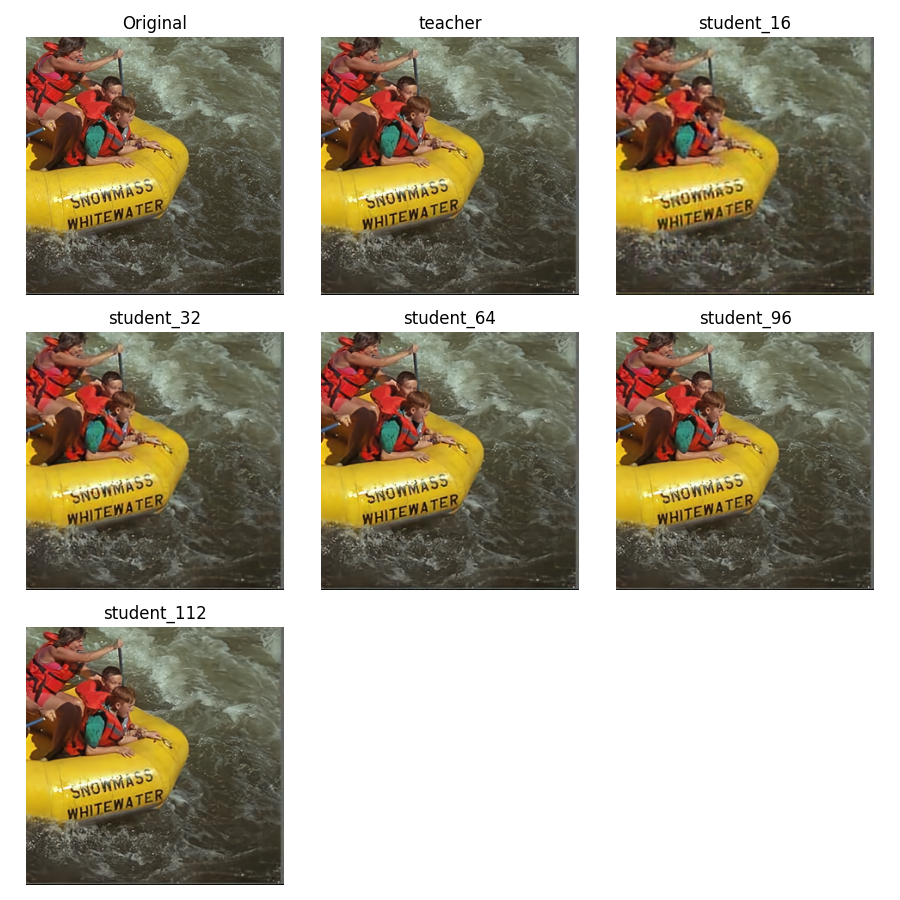
\includegraphics[width=8cm]{img/kd_ae_1.png} \label{kd_ae_1:a}}
    \qquad
    \subfloat[Pre-trained networks]{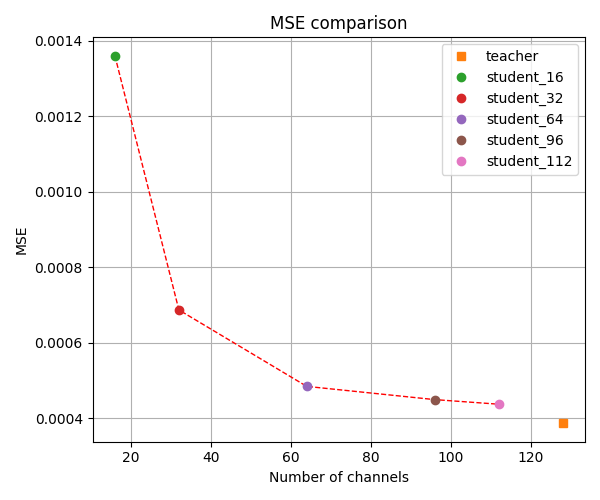
\includegraphics[width=8cm]{img/kd_ae_2.png} \label{kd_ae_1:b}}
    \caption[]{}
    \label{kd_ae_1}
\end{figure}

For reference, we show in Figure \ref{kd_ae_2} the \acrshort{rd} performances of the student models. It should be noted that the teacher network used in this experiment was trained for image compression tasks. One could argue that these models are not exactly auto-encoders for image reconstruction. What is sure is that they are far from state-of-the-art models in image compression tasks. What remains to be seen is to what extent a properly defined \acrshort{kd} loss for \acrshort{lic} does increase the \acrshort{rd} performance of these student models. This, as well as discussion related to the benefits of smaller student models for \acrshort{lic}, is the subject of the next section.

\begin{figure}
    \centering
    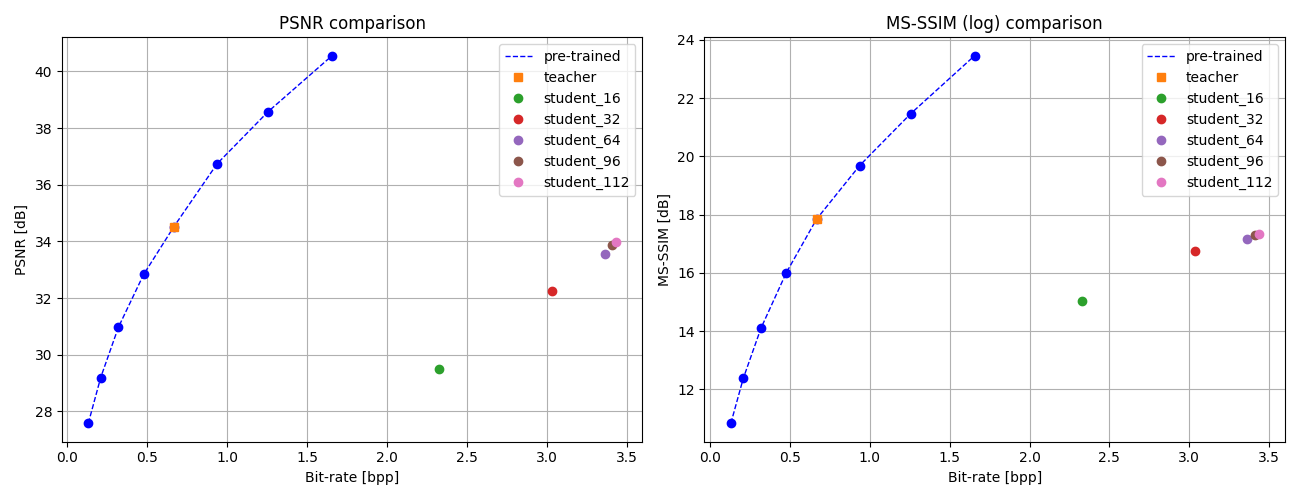
\includegraphics[width=15cm]{img/kd_ae_3.png}
    \caption[]{}
    \label{kd_ae_2}
\end{figure}

\section{Knowledge Distillation for Image Compression}
Having assessed the effectiveness of \acrshort{kd} for computer vision tasks similar to image compression, we investigate the success of this frugal \acrshort{ai} technique on image compression as defined by Ballé et al. in \cite{ballé2016endtoendoptimizationnonlineartransform}. Still using the scale hyperprior model introduced in \cite{ballé2018variationalimagecompressionscale}, we train a serie of student models with \acrshort{kd} to evaluate both their \acrshort{rd} perofrmance and their ability to be deployed on resource constrained platforms.

\subsection{Rate-Distortion Performance}
This part of the study focuses on training scale hyperprior models with \acrshort{kd} in order to achieve good \acrshort{rd} performance. We first explain our method then we present our results.

\acrshort{lic} distinguish itself from other computer vision tasks (such as dimensionality reduction) by minimising the entropy of the latent representation. In dimensionality reduction, the latent representation has no practical application. When it comes to image compression, it is the latent representation of the image that will be stored or transmitted. Having the smallest possible entropy allows for a smaller entropy coding which means less bits to handle during practical applications. This is why the rate-distortion loss is used in \acrshort{lic} as it allows to find the correct tradeoff between image quality and bit-rate according to the requirements of the application. In order to have similar results with \acrshort{lic}, the previous loss function (Equation \eqref{loss_1}) is updated as follow:

\begin{align}
    L &= \lambda_{1} MSE(z_{student}, z_{teacher}) + \lambda_{2} MSE(\hat{x}_{student}, \hat{x}_{teacher}) + \lambda_{3} RD(z_{student}, \hat{x}_{student}, x)\\
      &= \lambda_{1} MSE(z_{student}, z_{teacher}) + \lambda_{2} MSE(\hat{x}_{student}, \hat{x}_{teacher}) + \lambda_{3} (-E[\log_{2}P_{q}] + \lambda MSE(\hat{x}_{student}, x)) \nonumber
\end{align}

Following the exact same methodology as in Section \ref{part_2:hyperprior}, we train five new models using \acrshort{kd}. We use \(\lambda = 0.025\) in the \acrshort{rd} part of the loss, the same value used by the teacher model during its training.

[TODO: results] % Use 263674, 274457, 274461, 274464, 263691

\subsection{Application to Resource Constrained Platfroms}
Having proved the effectiveness of \acrshort{kd} for \acrshort{lic} tasks in terms of \acrshort{rd} performance, let us dive into the second apsect of this study: making \acrshort{lic} possible on resource-limited platforms. We have access to small models which \acrshort{rd} performances are on par with larger models. This section analyses these models from a resource stand point accross three main axis: memory, computing power and energy consumption.

Most resource constrained computers deal with a limited amount of memory. This limiting factor sometimes make them unsuitable for tasks requiring large models. As discussed previously, \acrshort{kd} applied to image compression models allows to use smaller models without degrading \acrshort{rd} performance. % Analyse number of parameters and memory footprint

Computers can only perform a certain amount of operations per unit of time. When dealing with mainstream hardware, the computing power required to use an image compression model like the scale hyperprior model is sufficient. However, when dealing with resource constrained devices, the latency might increase which goes against our objectives of realtime decompression. With too much latency, it is impossible too extend image decompression to video decompression. Here we focus on two metrics: the number of \acrfull{flop} (the number of floating-point operations carried out to run an inference) and the time required to perform inference. More precisely, ... % Analyse flops and inference time

Finally, most edge devices also have access to a limited amount of energy whether it is in time because they run on battery like smartphones or in power like \acrshort{iot} devices that run 24/7 and thus should not consume a lot of energy. This is why we focus on ... % Analyse energy consumption

% 1/ Memory (nb parameters + memory footprint)
% 2/ Compute (flops + inference time)
% 3/ Energy consumption

[TODO: results] % Use 263674, 274457, 274461, 274464, 263691